\chapter{Introduction}

% We are witnessing an ever-increasing trend in data production, thus leading to the so-called \emph{Big Data} era. 
% \note[Luca][notesyellow]{Espandere descrizione con esempi e brevi cenni storici}

In the last twenty years, we have witnessed an unprecedented and ever-increasing trend in data production. 
\citeA{hilbert2011world} dates the rise of this phenomenon back to 2002, with the beginning of the digital age.
Indeed, the transition from analog to digital storage devices enormously expanded the capacity of accumulating data, thus leading to the \emph{Big Data} era.

The term big data was first introduced in 1990s \cite{16, 17} and it is commonly adopted to describe data sets whose size exceeds the potential to manipulate and analyze them within reasonable time limits \cite{snijders2012big}.
However, the expression does not target any specific storage size but rather assumes a deeper meaning that goes well beyond the sheer amount of data points.
In fact, big data embrace a broad spectrum of data sources ranging from structured, semi-structured and, mostly, unstructured data \cite{dedic2016towards}.
Although multiple connotations have been attributed to the concept of big data over the years, a commonly shared definition is related to the so-called \emph{5 Vs} \cite{3}:

\begin{itemize}
    \item \textbf{Volume}: the actual quantity of generated data is huge, in the order of magnitude of terabytes and petabytes \cite{sagiroglu2013big}. More generally, it indicates amounts that are too large and complex to exploit conventional data storage and processing technologies;
    
    \item \textbf{Variety}: the data may come in several data types and from diverse origins. These include sources as sensors, social media, log files and more, plus they encompass heterogeneous formats like text, images, audio, video and so on; 
    
    \item \textbf{Velocity}: data are produced and/or processed at high rates \cite{kitchin2016makes}, typically nearly real-time;
    
    \item \textbf{Value}: data must carry valuable information that, if correctly analyzed, bring business value and profitable insights \cite{uddin2014seven};
    
    \item \textbf{Veracity}: data sources must be reliable and generate high-quality data that can produce value \cite{onay2018review, 33};


\end{itemize}


Nonetheless, the community has not reached a complete agreement on the big data definition \cite{22, kitchin2016makes}, with some authors suggesting moving their characterization from the intrinsic properties to the techniques adopted to acquire, store, share and analyze the data \cite{balazka2020big}.


Besides the modification of the storage supply,  multiple factors significantly enhanced data production and, hence, favored the rise of the big data era.
% the demand for storage space and computing power.
In the first place, the diffusion of the internet and the progress of computer technologies provided more processing capabilities and easier access to data, thus stimulating further their production.
Consequently, several stakeholders as big tech companies, traditional industries, governments, healthcare institutions and more started increasingly contributing to this growth.
Finally, the introduction of \emph{smart} everyday objects that not only receive but also produce data exponentially accentuated individual contributions to the total data produced.
Modern objects, in fact, are endowed with technologies that allow to collect data and share them via a network -- the so-called Internet of Things \cite{ashton2009iot} --, thus augmenting the production rate even more.
For instance, sensors measuring the status and operation are now commonly used in industrial machinery and household appliances to ease their control and automate maintenance.
The same paradigm is also influencing the direction of the personal items market in various ways.
% and, in turn, new use-cases emerge from their adoption. 
For example, some tech companies are recently investing in wearable devices like watches and glasses to enable the users to be always connected with a rapidly mutable environment, track their progress and explore the world in unparalleled manners thanks to virtual reality.
Furthermore, the solutions that digitization offers are being explored to respond to the emerging challenges of current times.
Think, for instance, of the urge for modernization of institutional processes posed by the pandemic. The massive spread of the infections has required unprecedented amounts of patients needing access to health assistance. However, the impossibility to scale up services and equipment correspondingly caused huge issues and jeopardized people's safety. In such context, the availability of intelligent systems capable of remotely monitoring patients' conditions and providing them with specialist support would have enormously helped.

In order to cope with the growing amount of data to store and process, the big data players of both industry and academy have gradually moved to new computing paradigms in recent years. 
For instance, new solutions as \textbf{distributed} and \textbf{cloud computing} \sidenote[Luca][notesyellow]{Spiegare più approfonditamente?} have been specifically designed to address these new requirements, taking advantage of multiple resources geographically displaced and accessible via a network.

However, the boost in performance guaranteed by these technologies comes with the price of requiring very complex interactions of both hardware and software components. 
Aside from the enormous benefits these solutions bring, their most relevant drawback is that the wider the infrastructure, the higher the chances of something going wrong, and the bigger the effort to detect, inspect and solve the issues.
\Cref{partII} explores this domain and tries to propose a data-driven pipeline to ease and support people working to maintain the infrastructure integrity.
Despite applying to many different applications with some tuning, the presented approach is discussed in the context of \textbf{data transfer failures} within the \emph{Worldwide Large Hadron Collider Computing Grid} (WLCG).

\section{Background}
\begin{figure}
    \centering
    \subfloat[LHC accelerator]{
    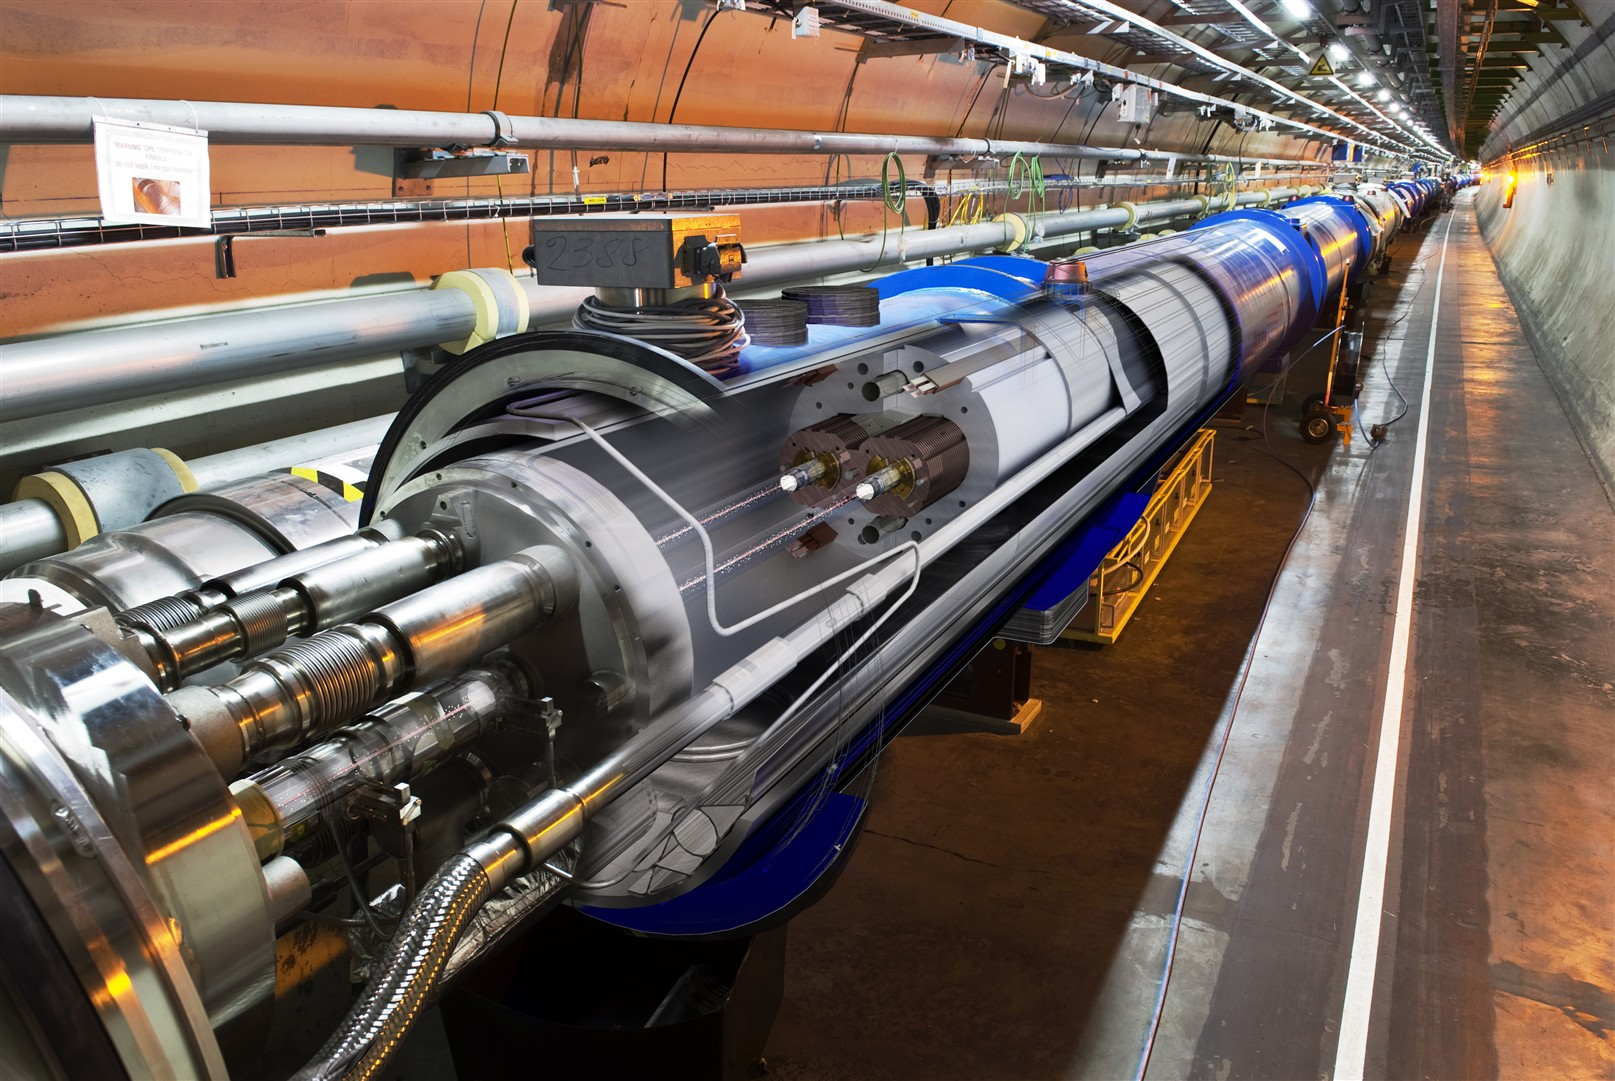
\includegraphics[width=\textwidth]{figures/220_introduction/cern/a0lhcinternotubo_445034351.jpg}
    }
    
    \subfloat[Aerial view]{
    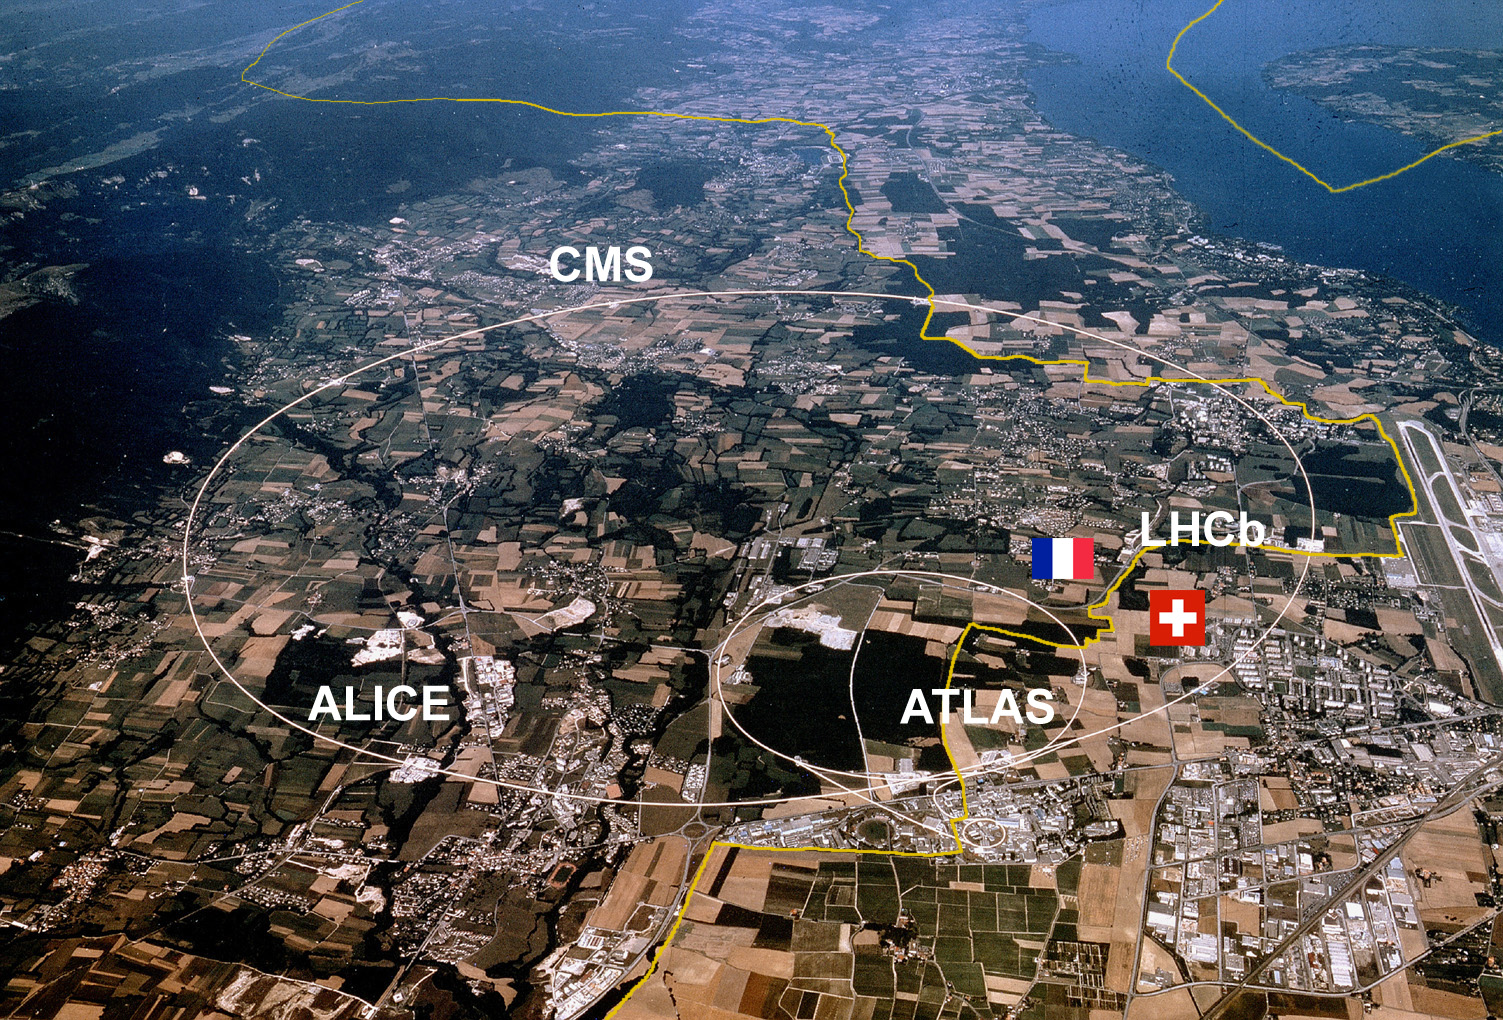
\includegraphics[width=0.5\textwidth]{figures/220_introduction/cern/CERN_location.jpg}
    }
    \subfloat[LHC scheme]{
    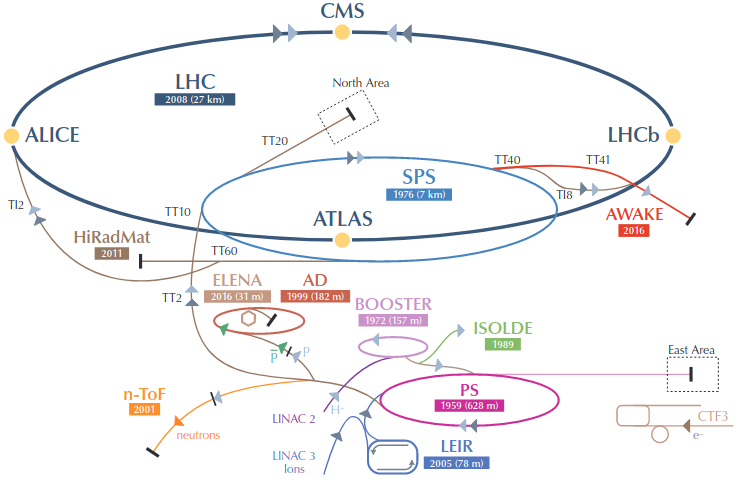
\includegraphics[width=0.5\textwidth]{figures/220_introduction/cern/lhc_scheme_factsfigures.png}
    }
    \caption{\textbf{LHC accelerator complex.} Top: the underground tunnel that hosts LHC and a transversal section of the pipes that compose it. 
    Bottom: aerial view of LHC complex at the boundary between Switzerland and France (left) and structure of the various accelerating structures that compose LHC (right).
    }
    \label{fig:lhc}
\end{figure}

\begin{figure}
    \centering
    \subfloat[ATLAS]{
    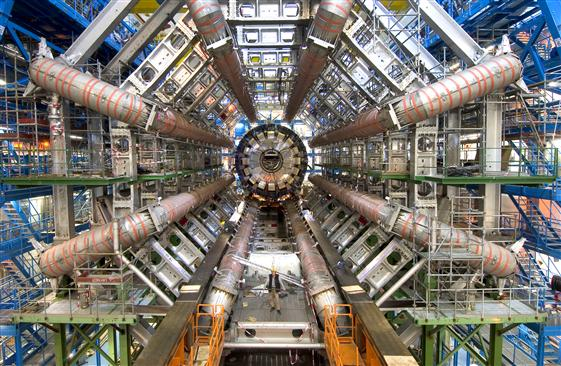
\includegraphics[width=0.5\textwidth]{figures/220_introduction/cern/atlas_detector_medium.jpg}
    }
    \subfloat[LHCb]{
    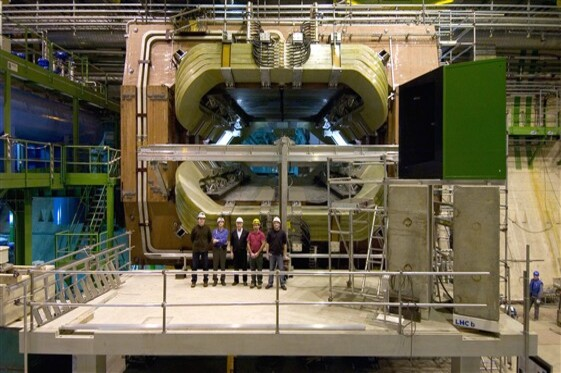
\includegraphics[width=0.5\textwidth]{figures/220_introduction/cern/lhcb_detector_medium.jpg}
    }
    
    \subfloat[ALICE]{
    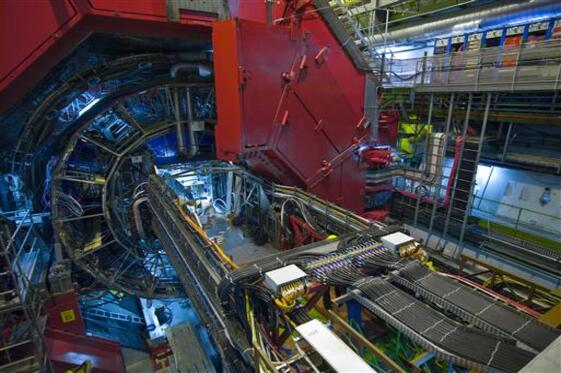
\includegraphics[width=0.5\textwidth]{figures/220_introduction/cern/alice_detector_medium1.jpg}
    }
    \subfloat[CMS]{
    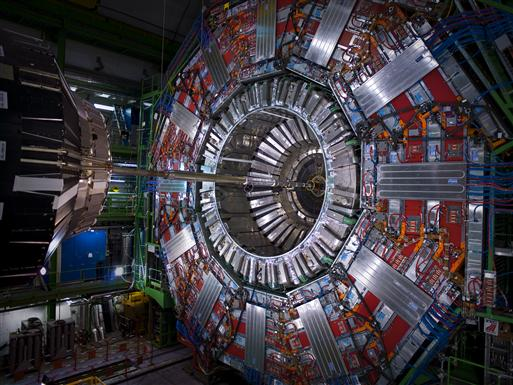
\includegraphics[width=0.5\textwidth]{figures/220_introduction/cern/cms_detector_medium.jpg}
    }
    \caption{\textbf{CERN 4 major experiments.}}
    \label{fig:cern_experiments}
\end{figure}

\note[Luca][notesyellow]{Introduction to HEP community, with mention to WLCG as an essential tool to perform their research}

% High-Energy Physics (HEP) is a branch of physics that studies the fundamental constituents of matter and the forces that drive their interactions. One of the methods is to create very high energy densities. 
% This reproduces the environmental conditions of the primordial universe.

High-Energy Physics (HEP) is a branch of physics that studies the elementary constituents of matter and the fundamental principles that govern their interaction to understand how our universe has formed and evolved.  
These particles, however, are not visible at the scales whereby we experience reality today. 
Thus, HEP experiments need to either look at natural phenomena generated in pressure and temperature conditions similar to those of the primordial universe -- like cosmic rays -- or recreate such settings artificially.

The European Council for Nuclear Research (CERN) is part of this second strand of experiments, and it constitutes the largest particle physics laboratory in the world.
From 2008, CERN facilities also include the Large Hadron Collider (LHC), the longest particle accelerator ever built.
LHC consists of a \mbox{26.7-kilometer} ring located in a tunnel about 100 meters underground in the Geneva area (\cref{fig:lhc}), and it is made of superconducting magnets with several accelerating structures \cite{lhcwebsite}.
Inside the accelerator, bunches of protons are revved up to nearly the speed of light, forming two high-energy particle beams that travel in opposite directions inside separated pipes. 
When they acquire the desired energy, the beams are directed towards dedicated interaction points where the experiments occur. %surrounded by giant detectors.
In practice, LHC hosts four major experiments built in correspondence of these locations -- ATLAS \cite{aad2008atlas}, ALICE \cite{aamodt2008alice}, LHCb \cite{alves2008lhcb} and CMS \cite{collaboration2008cms} -- and equipped with giant detectors (\cref{fig:cern_experiments}).
Once the beams get there, the two pipes cross and the particles are squeezed through substantial magnetic fields to increase their chances of colliding. 
In this way, a massive amount of energy is concentrated in an extremely tiny area, generating millions of particles at each collision.
Indeed, the high speed of the beams causes roughly 40 million crossings per second at each interaction point \cite{albrecht2019roadmap, grandi2017HEPsize}. 
\sidenote[Luca][notesyellow]{Controllare numeriche ed aggiungere reference}
When a crossing happens, an average of 60 bunch collisions -- also referred to as pileup -- are observed \cite{albrecht2019roadmap}. The particles produced by each scattering then fly around the interaction point to be eventually detected through high-technology experimental devices endowed with over 100 million electronic channels \cite{grandi2017HEPsize, aad2020channels}.
According to the latest experimental setup, this delivers 100 MegaBytes (MB) of data per collision and it would generate 40k ExaBytes (EB) every year \cite{grandi2017HEPsize}.
However, storing such a tremendous amount of data is unattainable with current technology and budget. In addition, the events of interest are typically rare, so there is actually no need to record all of the information detected by the electronic channels.
Thus, the vast majority of \emph{read-out} data from collisions is discarded straight away and the \emph{recorded} event rate is lowered to 1k crossings per second. 
As a result of this reduction, the actual acquisition rate
% amounts to 1MB every second, translating to roughly 100 PetaBytes (PB) a year in 2018 \cite{grandi2017HEPsize, altre?}.
amounts to nearly 1 PB per day \cite{cern2017storage}, translating to roughly 160 PetaBytes (PB)%
\footnote{LHC registered 161 days of physics data taking in 2018 \cite{todd2018lhcAvail}}
a year in 2018. %\cite{grandi2017HEPsize, cern2017datayear}.
Besides that, physics analyses require comparing experimental results with Monte Carlo data simulated according to current theories, thus producing somewhat between 1 and 2 times additional data \cite{grandi2017HEPsize}.
Furthermore, the CERN community is already working at enhancing the Large Hadron Collider capabilities.
The project involves boosting the energy of the beam and gradually increasing the pileup towards 200 collisions per bunch crossing \cite{albrecht2019roadmap}, thus leading to the so-called High Luminosity LHC (HL-LHC) \cite{hllhc}.
% Thanks to this upgrade, way more events will be observed as the beam energy will be boosted and the pileup will gradually be increased towards 150 collisions per bunch crossing.
% In this new regime, 
Thanks to this upgrade, the observed events are expected to increase of a factor $\geq5$\cite{giuspe2021tesi} and produce an estimated 800 PB of new data each year by 2026.%\cite{grandi2017HEPsize, HLLHC_data}.

Although it is difficult to replicate such a punctual measurement of the data production for other big data players, some hints can be retrieved by comparing multiple online resources. %\cite{BDPlot_series}. 
\Cref{fig:bidata_size} tries to summarize a reasonable, up-to-date ``guesstimate"%
\footnote{These data are reconstructed based on multiple online sources about the amount of contents produced, streamed or hosted by big data companies and reasonable estimates of unitary sizes for such contents, e.g. average mail or picture size, average data traffic for 1 hour video, and so on. 
However, the actual values reported are not meant to be extremely accurate and only serve the purpose of giving an idea of the orders of magnitude of the various phenomena.
}
of yearly data production for the main big data companies.
Despite not being the most popular among the mainstream audience, the HEP community is one of the most prominent players concerning big data.
% \begin{landscape}
% \begin{figure}
%     \centering
% \begin{tikzpicture}%[shorten >=1pt,node distance=1cm,on grid,auto] 
% \linespread{.5}%
% \begin{scope}
%     \node[anchor=south west,inner sep=0] (image) at (0,0){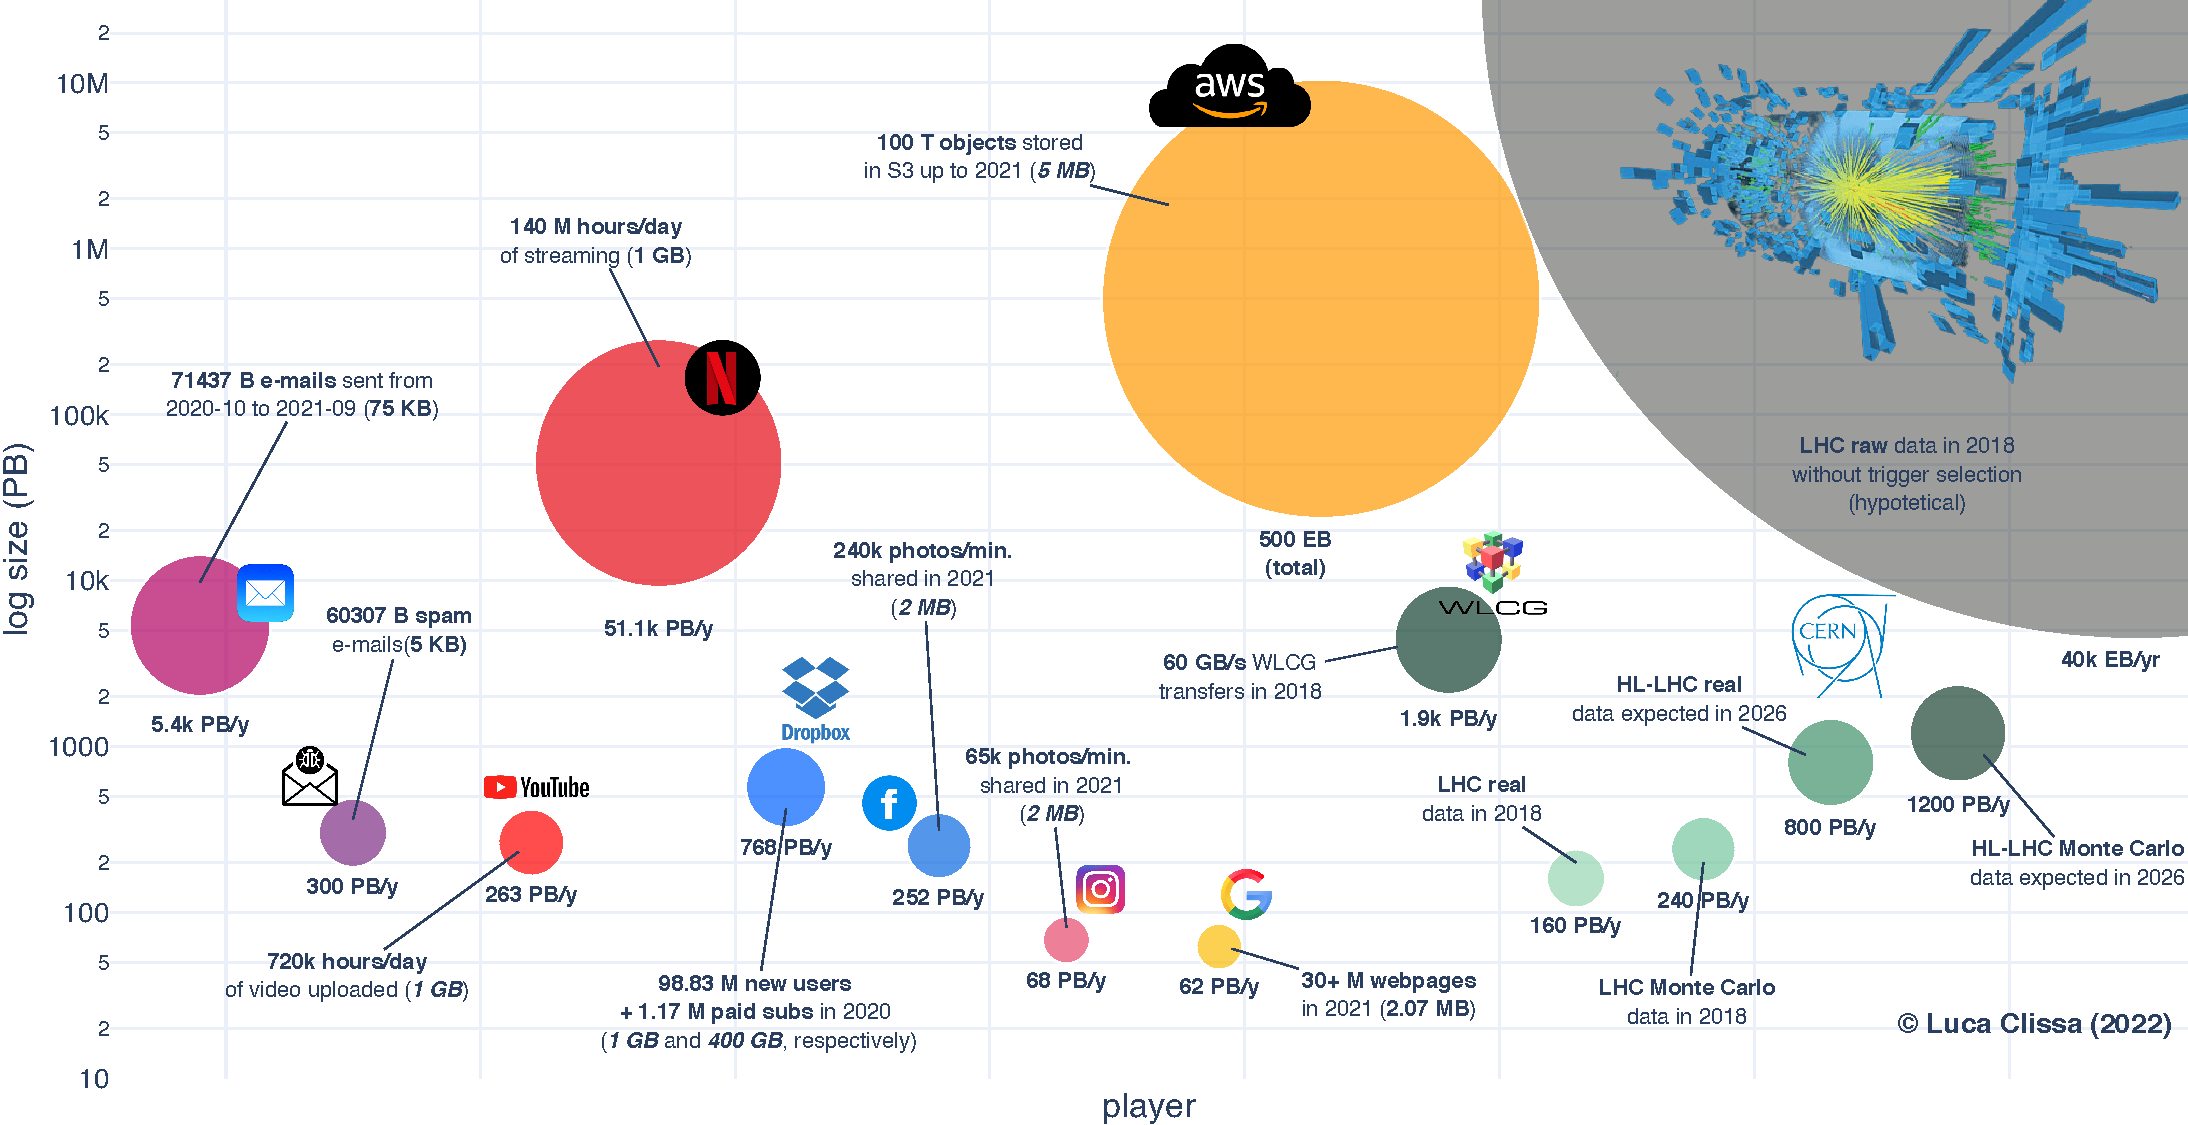
\includegraphics[width=\linewidth]{figures/220_introduction/BigData2021.pdf}};
% \begin{scope}[x={(image.south east)},y={(image.north west)}]
%     \node [anchor=west] (note1) at (0.26,0.170) {\href{https://stackoverflow.com}{Link}};
%         \node [anchor=west, scale=1, align=center,font=\tiny] (note2) at (0.26,0.470) {\href{https://rdcu.be/cB1Ds}{paper} \\ from the future};
% \end{scope}
%     \end{scope}
% \end{tikzpicture}
% \caption{\textbf{Big Data sizes.} Bubble plot of the orders of magnitude of data produced by important big data players. The balloon areas illustrate the amount of data and the text annotations highlight the key factors considered in the estimates. Average per-unit-sizes are reported in parentheses, where italic indicates measures reconstructed based on likely assumptions because no references were found.} \label{fig:bidata_size1}
% \end{figure}
% \end{landscape}
\begin{landscape}
\begin{figure}
    \centering
    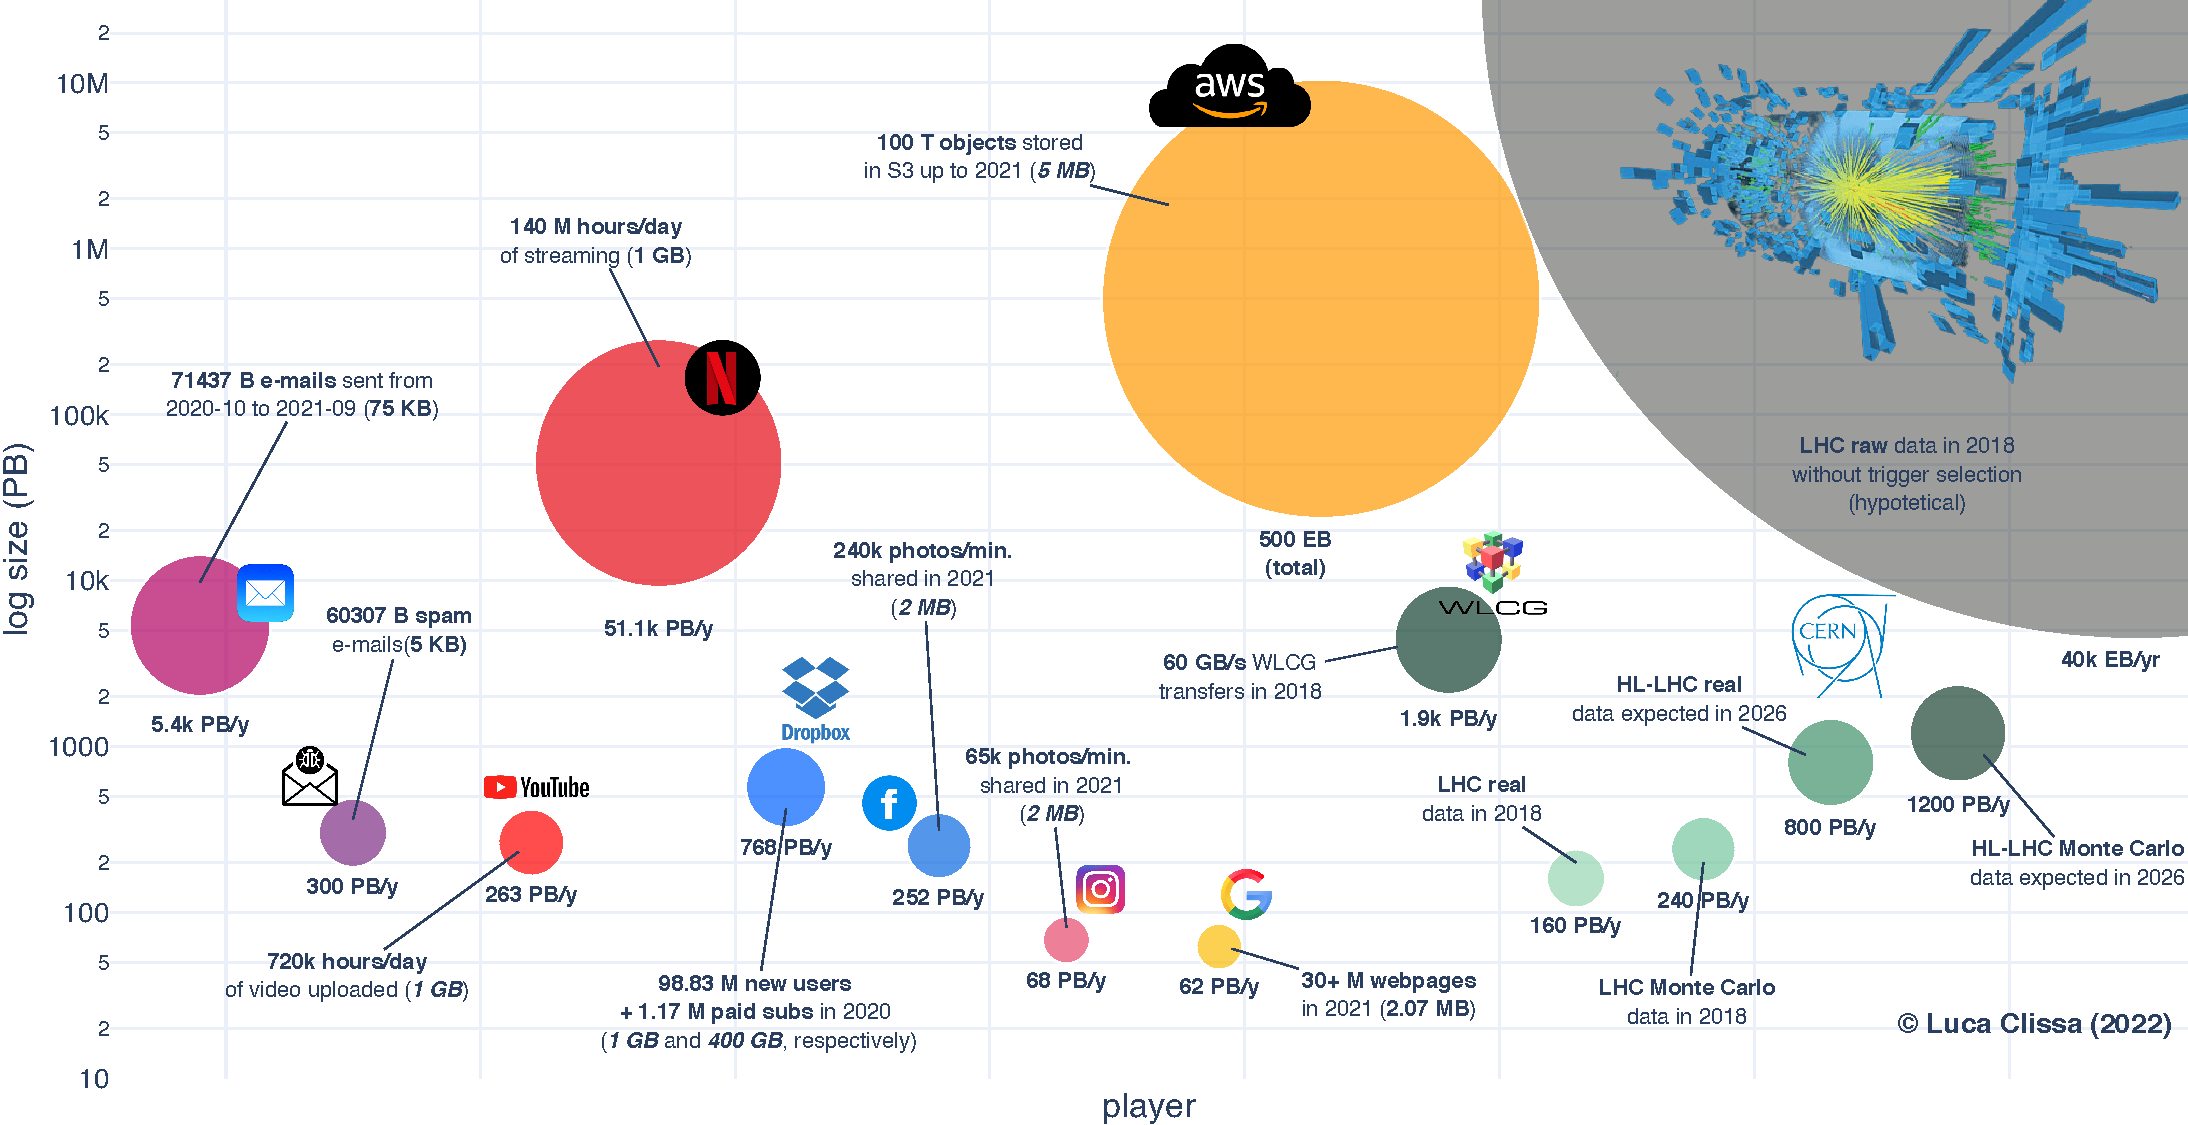
\includegraphics[width=\linewidth]{figures/220_introduction/BigData2021.pdf}
    \caption{\textbf{Big Data sizes.} Bubble plot of the orders of magnitude of data produced by important big data players. The balloon areas illustrate the amount of data and the text annotations highlight the key factors considered in the estimates. Average per-unit-sizes are reported in parentheses, where italic indicates measures reconstructed based on likely assumptions because no references were found. Interactive version available at: \href{https://clissa.github.io/BigData2021/BigData2021.html}{BigData2021.html}}
    \label{fig:bidata_size}
\end{figure}
\end{landscape}

Indeed the read-out data LHC produced every year in Phase 2 (40k EB) is around one order of magnitude bigger than the total size of objects ever stored on Amazon AWS cloud service (500 EB)%
\footnote{Obtained considering the total number of objects reportedly stored in Amazon S3 (100 trillion, \citeA{amazon2021objectscount}) and assuming an average size of 5 MB based on some average bucket example \cite{amazon2021objectssize}}.
Considering effectively recorded data, LHC figures are comparable with those of other most renowned big data entities. The last run (2018), in fact, produced hundreds of PetaBytes (PB) (roughly 160 of real data and 240 of Monte Carlo simulations),
 which is similar to the orders of magnitude generated by Google searches (62 PB)%
\footnote{Obtained considering that Google search index contains at least 30 billion webpages \cite{van2016estimating, google2021index_size, djuraskovic2020googl_stats, indig2020index_size} and that the average page size is 2.07 MB \cite{http2021webpage_size}
},
Instagram and Facebook shared photos (68 and 252 PB, respectively)%
\footnote{Obtained considering that 65k and 240k pictures are shared every minute on Instagram and Facebook \cite{domo2021infographic}, and assuming 2 MB as a reasonable average picture size \cite{adobe2021fb_img_size}
}
and YouTube video uploads (263 PB)%
\footnote{Obtained considering that 720k hours of video are uploaded daily \cite{domo2021infographic} and assuming an average size of 1 GB \cite{quora2021youtube}
}.
Moreover, LHC will climb the table even further with the upgrade to high luminosity, when the real and Monte Carlo data production rate is expected to rise to levels comparable to those of storage services like Dropbox (800, 1200 and 768 PB%
\footnote{Obtained considering that Dropbox registered 100 million of new users in 2020, of which 1.17 million were paid subscriptions \cite{dean2021dropbox}. For the average per-unit-size, it was assumed that free accounts exploited 75\% of the 2 GB storage available, while paid ones exploited 25\% of the total 2 TB
}, respectively). 

Apart from the nominal values of the generated information, streaming data comprise a significant slice of the big data market.
As a matter of fact, the continual movement of small- to medium-sized files spawns massive traffic when scaled up to millions of users, as testified by e-mails (5.7k PB)%
\footnote{Obtained considering that 71k billion e-mails and 60k billion spam messages were sent from October 2020 to September 2021 \cite{statista2021mails}, and that the average size is \mbox{75 KB} for e-mails \cite{lifewire2021avg_mail} and \mbox{5} KB for spam \cite{medium2014avg_spam}
},
and Netflix (51.1k PB)%
\footnote{Obtained considering that Netflix users consumed 140 million hours per day of streaming \cite{domo2021infographic} and that counts for 1 GB of data for standard definition videos \cite{perry2021netflix}
} bubbles in \cref{fig:bidata_size}.
% Also in this respect, LHC plays an important role. Indeed, the HEP community is formed by thousands of researchers spread around the world that need to access the data produced at CERN.
A similar usage is generated also by the LHC, whose data are continuously transferred across the HEP community thanks to the Worldwide LHC Computing Grid (see \cref{wlcg}) to fuel innovative research. For example, 
% 12 PB of data were accessed on average every day in 2020 for the ATLAS experiment alone \cite{calafiura2020design_report}, and
a throughput of 60 GB/s was generated by the 4 experiments together in 2018 \cite{wlcg2018throughput} thus giving a yearly projection (1.9k PB) close to half of the global e-mails traffic and only one order of magnitude lower than Netflix usage.
% Indeed, thousands of researchers from all around the world need to access LHC data, analyze them and share their results to investigate new theories and advance our knowledge of the universe.
% For this reason, the Worldwide LHC Computing Grid computing infrastructure has been developed over the years 

Given the large quantities of data involved by the LHC, it is not surprising how careful planning must be done in order to meet the needs of the LHC community, and tailored strategies and technologies must be adopted to cope with such requirements. 
Luckily, the presence of other stakeholders facing analogous problems provides the HEP community with some alternatives to draw from, and it allows researchers to tap in from existing solutions and customize them for their necessities.

\subsection{The Worldwide LHC Computing Grid}
\label{wlcg}

\sidenote[Luca][notesyellow]{Cos'è WLCG?}
The Worldwide LHC Computing Grid (WLCG) is a global collaboration that links up more than 170 computing centers in 42 countries. 
As of today, WLCG constitutes the largest computing grid in the world and it is supported by many associated national and international grids across the world, such as European Grid Initiative (Europe-based) and Open Science Grid (US-based), as well as many other regional grids.

Founded in 2002 by CERN, the WLCG mission is to provide computing resources to store, distribute and analyze the data generated by the Large Hadron Collider (LHC).
In order to do that, WLCG leverages a distributed computing paradigm to share resources -- in terms of infrastructures, personpower and fundings -- among member states and make them equally available to all the partners, regardless of their physical location.

WLCG is the world's largest computing grid. It is supported by many associated national and international grids across the world, such as European Grid Initiative (Europe-based) and Open Science Grid (US-based), as well as many other regional grids.

WLCG is co-ordinated by CERN. It is managed and operated by a worldwide collaboration between the experiments (ALICE, ATLAS, CMS and LHCb) and the participating computer centres. It is reviewed by a board of delegates from partner country funding agencies, and scientifically reviewed by the LHC Experiments Committee.

\sidenote[Luca][notesyellow]{Cosa fa WLCG?}
WLCG provides seamless access to computing resources which include data storage capacity, processing power, sensors, visualization tools and more. Users make job requests from one of the many entry points into the system. A job will entail the processing of a requested set of data, using software provided by the experiments

The computing Grid establishes the identity of the user, checks their credentials, and searches for available sites that can provide the resources requested. Users do not have to worry about where the computing resources are coming from – they can tap into the Grid's computing power and access storage on demand.


\sidenote[Luca][notesyellow]{WLCG community}
The Worldwide LHC Computing Grid (WLCG) is a distributed computing infrastructure arranged in tiers – giving a community of over 12,000 physicists near real-time access to LHC data. Data pours out of the LHC detectors at a blistering rate. Even after filtering out 99\% of it, in 2018 we gathered 88 petabytes of data. That's 88 million gigabytes, the equivalent to around 22 million high-definition (HD) movies.

\sidenote[Luca][notesyellow]{Cos'è WLCG?}
The scale and complexity of data from the LHC is unprecedented. This data needs to be stored, easily retrieved and analysed by physicists all over the world. This requires massive storage facilities, global networking, immense computing power, and, of course, funding.

\sidenote[Luca][notesyellow]{Inserire qui una descrizione dell'infrastruttura}

\sidenote[Luca][notesyellow]{Ordini di grandezza}
The next LHC Run is scheduled for 2021-2023. This looks to be even more challenging than the previous runs; data archiving is expected to be double what it was for LHC Run 2, and Run 4 - in HL-LHC operation - is even expected to be fives times that. 

The requirements for data and computing will grow dramatically during this time, with rates of 500 PB/year expected for the HL-LHC. The needs for processing are expected to increase more than 10 times over and above what technology evolution will provide. As a consequence, partnerships such as those with CERN openlab and other programmes of research and development are essential to investigate how the computing models could evolve to address these needs. They will focus on applying more intelligence into filtering and selecting data as early as possible. Investigating the distributed infrastructure itself (the grid) and how one can best make use of available technologies and opportunistic resources (grid, cloud, HPC, volunteer, etc), improving software performance to optimise the overall system.








$$\dots$$

% One of the biggest collaborations working on distributed computing is the WLCG. 
% The LHC grid has a very layered topology, both in terms of physical organization and of ...
% is made of many services, each taking care of specific sub-processes that together enables the global functioning of the whole infrastructure.
\sidenote[Luca][notesyellow]{Explain why data are moved around by these communities}
In such a vast environment, a great deal of attention is devoted to the data, which are arguably the most valuable good of the community.
For example, specific distribution and redundancy policies have been set to prevent data loss. Also, a careful design is put in place to guarantee a FAIR access to them.
In particular, data must be available at any time for researchers to analyse them and contribute to the progression of science in their sectors.
\sidenote[Luca][notesyellow]{introduce transfer failures}
Consequently, massive amounts of data -- both in size and number -- are frequently moved across the grid, occasionally experiencing failures ranging from a user mistyping a command to more severe software/hardware defects that require prompt intervention. 
For this reason, data transfer processes are continuously monitored by teams of shifters whose job is to detect issues and report them to experts that take care of their solution.
\lc{Here goes some reference to the orders of magnitude at stake, i.e.: 
\begin{itemize}
    \item n. tranfers/day (whole or per virtual organization) --> can retrieve from FTS
    \item ticket/year or month or day (whole or per virtual organization) --> how to retrieve that? is there any official source?
\end{itemize}
}

Due to the complexity of the infrastructure and its layered structure, identifying potential problems, understanding their causes and fixing them may take a while, thus demanding a great human effort.
\lc{Describe current operations and possibly volumes: 
\begin{itemize}
    \item Current operations: efficiency matrix + drill down (description + falls)
    \item average solving time $\rightarrow$ how to retrieve that? is there any official source?
    \item n. people involved (both shifters and sites) $\rightarrow$ how to retrieve that? is there any official source?
\end{itemize}
}
%Current operations are based on a site-centric monitoring approach that involves mainly manual, post-mortem reporting. In this approach, trained operators look at Grafana dashboards that act as a high-level overview of the systems status and try to spot hints of incorrect or undesired behaviours.
Current operations are based on a site-centric approach where trained personnel monitor the status of the various services almost 24/7 and try to spot hints of incorrect or undesired behaviours. In particular, they look at Grafana dashboards acting as a high-level overview of the system. A usual starting point is the so-called efficiency matrix (Figure \ref{fig:efficiency_matrix}), where the percentage of successful transfers is reported at customisable levels ranging from cloud to site, endpoint or even space token.
\begin{figure}
    \centering
    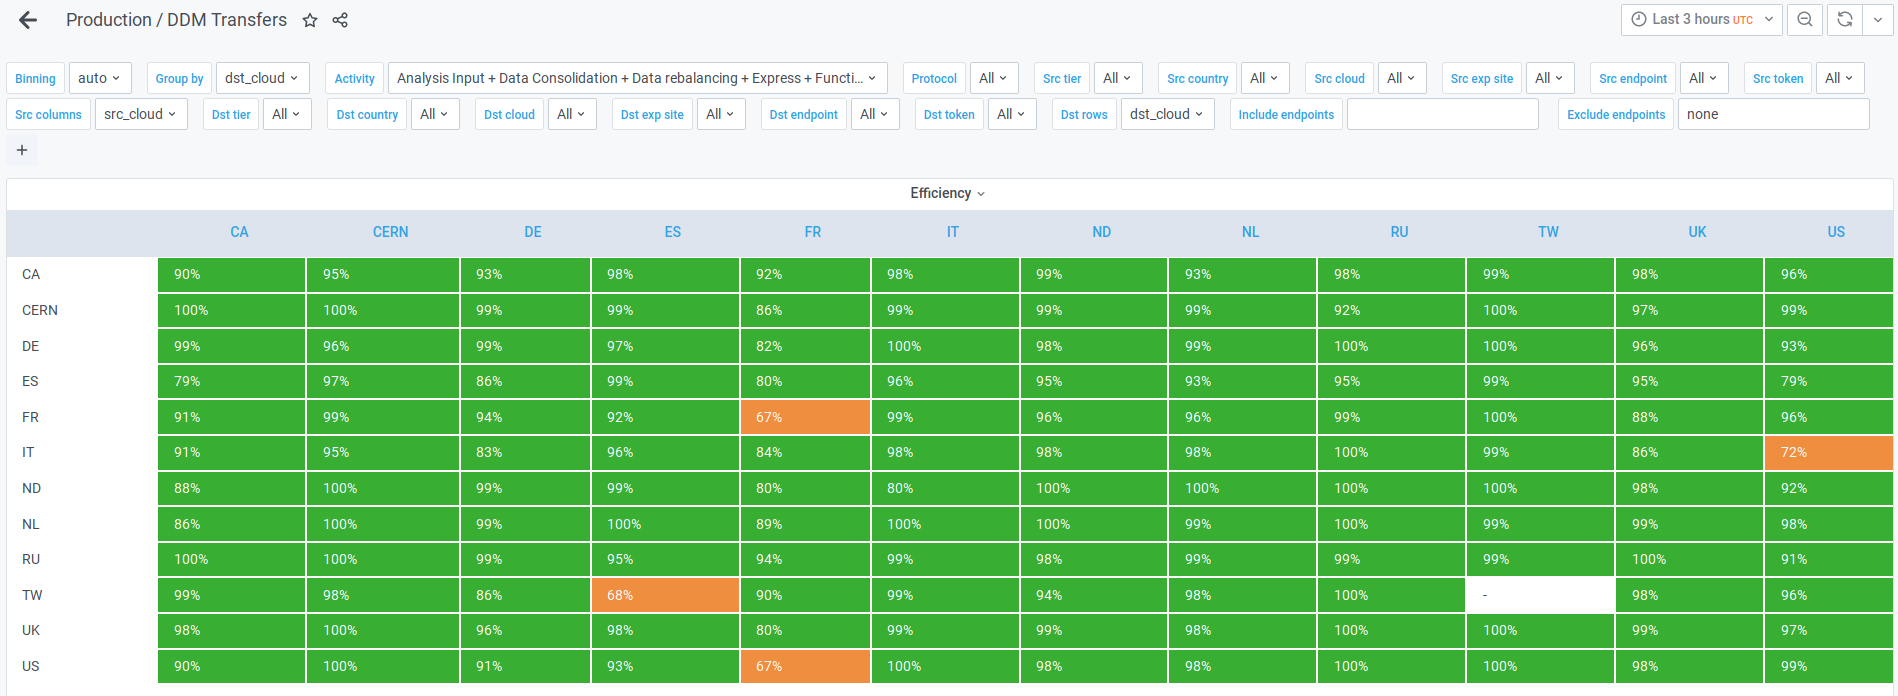
\includegraphics[width=\textwidth]{figures/220_introduction/efficiency_matrix.png}
    \caption{Transfer efficiency matrix from Grafana. Transfer sources are shown as columns and destinations as row. The drop-down menus at the top allow custom filtering.}
    \label{fig:efficiency_matrix}
\end{figure}
When the efficiency falls below an acceptable threshold, typically 60-70\%, on-duty shifters start to investigate the issue at a lower level by checking \emph{i)} where the error happened, \emph{ii)} how many errors are produced, \emph{iii)} what is the time pattern (temporary, extended or cyclical) and \emph{iv)} which error messages are generated. 
However, this procedure gives rise to many false alarms as it is usual to encounter problems that do not represent a real concern. This typically happens when the failure rate is high because just a few transfers were attempted, or there was a transient issue that was already fixed. 
Also, sometimes unnecessary drill-down activity is performed for actual issues that were already known, as in the case of ongoing tickets or site downtimes, for which reporting is not required.
As a result, many human resources are employed in repetitive tasks of little scientific interest that would enormously benefit from automation. 

\sidenote[Luca][notesyellow]{Describe also why a site-centric approach is not optimal and how a message-centric one could help}
In addition to that, a site-centric strategy as described above has some drawbacks. Firstly, monitoring focuses on spotting where issues occur, while understanding the actual root causes is typically demanded to site experts in a subsequent investigation.
Secondly, problems generating few error messages are usually ignored. This is natural, and to some extent desirable, as having limited resources forces us to address bigger misfunctioning first. However, that could be a potential pitfall in cases where promptly fixing a minor issue may prevent the rising of a more significant and longer to solve defect.

All these problems could be tackled programmatically by standardising the logging output of all the services. In this way, neat error messages would point directly to the source of the problem, thus allowing complete automation. 
However, the distributed nature of the infrastructure hampers such an approach.
In fact, the opportunistic gathering of computing resources that led to WLCG entails many local configurations that are not easy to address using only a static strategy.
Hence, all these considerations expose the need for an intelligent support tool for speeding up infrastructure management to meet the productivity requirements for the near future.

% Hence, the current approach will no longer meet the productivity requirements in the near future given the limited resources

\subsection{Contribution}
The goal of this work is to discuss a complementary, experiment-agnostic, computer-aided approach to grid monitoring centered on error messages rather than site performances.

In particular, we propose an unsupervised Machine Learning (ML) pipeline to identify clusters of similar failures. These groups are then exposed to shifters as suggestions of potential issues to investigate further.